% Provenance (never printed): sources/book2/BRIEFS.md, g11-02. Production function, diminishing marginal
% product, the cost family, the long run (scale), the learning curve. Real numbers: figdata/grade-11/
% 02-production-and-costs/ (WDI cereal yield and fertiliser use, 2018-2020; Duflo, Kremer and Robinson 2008
% Table 1 as a cited table). Ledger: DKR2008 rows, Liberty ships (Thompson 1997, reporting Searle 1945).
% The Liberty-ship monthly chart of the brief was dropped (the launch photograph is in, Commons, PD): no monthly table was
% available from an approved or citable source (Searle 1945 issue too large to fetch); the record box gives
% the yard-level figures instead. Kestria's textile mill and the workshop numbers are invented.
\chapter{Production and Costs}\label{ch:g11:production-and-costs}

In 2018--2020 farmers in Kenya spread on average about 52 kilograms of fertiliser on each hectare of arable land, and harvested about 1.7 tonnes
of cereals a hectare. In the Netherlands they spread about 275 kilograms and harvested 8.2 tonnes. Across 179 countries, the curve that best fits
the points says that going from 20 to 21 kilograms of fertiliser a hectare goes with about 53 more kilograms of grain, and going from 200 to 201
with about 5.
% figdata: cereal_marked (KEN 51.9, 1719; NLD 274.9, 8183); cereal_fit (n 179, mp20 53.3, mp200 5.3)

The countries differ in much more than fertiliser: in rain, soil, seeds, irrigation and machines. The curve cannot say how much of the gap the
fertiliser explains. Field trials in which only the fertiliser changes, met later in this chapter, show the same shape: each extra spoonful adds
less than the one before. This is the first fact about production, and the costs of every firm follow from it.

\begin{openingchart}{Cereal yield against fertiliser use, 179 countries, means of 2018--2020. Fertiliser is in kilograms a hectare of arable land,
on a times-ten scale. The curve is the line, on this scale, that passes closest to the points.}{World Bank, World Development Indicators: cereal
yield (kg per hectare); fertilizer consumption (kilograms per hectare of arable land)}
\begin{tikzpicture}
\begin{semilogxaxis}[omscatter, log basis x=10, log ticks with fixed point, xtick={1,10,100,1000}, width=0.84\linewidth, height=6.6cm,
  xmin=0.5, xmax=2000, ymin=0, ymax=12000, scaled y ticks=false, yticklabel style={/pgf/number format/fixed, /pgf/number format/1000 sep={\,}},
  xlabel={fertiliser (kg a hectare)}, ylabel={cereal yield (kg a hectare)}]
\addplot[omDef, only marks, mark=*, mark size=1.2pt, fill opacity=0.7]
  table[x=fert, y=yield] {figdata/grade-11/02-production-and-costs/out/cereal.csv};
\addplot[black, thick, no markers, sharp plot] table[x=fert, y=yield] {figdata/grade-11/02-production-and-costs/out/cereal_curve.csv};
\addplot[omThm, only marks, mark=square*, mark size=1.8pt]
  table[x=fert, y=yield] {figdata/grade-11/02-production-and-costs/out/cereal_marked.csv};
\node[font=\scriptsize, text=omThm!80!black, anchor=south east] at (axis cs:131.7,8115) {USA};
\node[font=\scriptsize, text=omThm!80!black, anchor=south west] at (axis cs:274.9,8183) {NLD};
\draw[omThm!60] (axis cs:428.3,6234) -- (axis cs:1100,9500) node[anchor=south, font=\scriptsize, text=omThm!80!black] {CHN};
\draw[omThm!60] (axis cs:190.6,3362) -- (axis cs:900,1200) node[anchor=west, font=\scriptsize, text=omThm!80!black] {IND};
\draw[omThm!60] (axis cs:51.9,1719) -- (axis cs:9,4800) node[anchor=south, font=\scriptsize, text=omThm!80!black] {KEN};
\end{semilogxaxis}
\end{tikzpicture}
\end{openingchart}

\begin{recall}
From the grades 6--9 volume: a firm's \emph{revenue} is what it sells times the price, its \emph{fixed costs} do not change with the quantity it
produces and its \emph{variable costs} do; \emph{productivity} is output per unit of input. From \cref{ch:g11:marginal-reasoning}: \omterm{def:g11:marginal-reasoning:marginal-benefit}{marginal cost}, and
\cref{prop:g11:marginal-reasoning:average} (the marginal pulls the average). From mathematics: the derivative of a quotient.
\end{recall}

\section{The production function}\label{sec:g11:production-and-costs:function}

\begin{definition}[Production function]\label{def:g11:production-and-costs:production-function}
A \emph{production function}\index{production function} gives the largest output that a firm can produce from given quantities of its inputs (labour,
machines, buildings, land, materials).
\end{definition}

\begin{definition}[Fixed and variable inputs; short and long run]\label{def:g11:production-and-costs:fixed-input}
A \emph{fixed input}\index{fixed input} is one whose quantity the firm cannot change within the period considered; a \emph{variable input}\index{variable input}%
\phantomsection\label{def:g11:production-and-costs:variable-input} is one it can. The \emph{short run}\index{short run}%
\phantomsection\label{def:g11:production-and-costs:short-run} is a period in which at least one input is fixed; the \emph{long run}\index{long run}%
\phantomsection\label{def:g11:production-and-costs:long-run} is a period long enough for every input to be changed.
\end{definition}

A bakery with one oven can hire more bakers this week, but it needs months to install a second oven. With the oven fixed, its output depends on the
number of bakers $L$ alone: $Q = f(L)$.

\begin{definition}[Marginal product]\label{def:g11:production-and-costs:marginal-product}
The \emph{marginal product}\index{marginal product} of an input is the extra output from one more unit of it, the other inputs being held fixed: $f(L + 1) -
f(L)$, or $f'(L)$ when $f$ is differentiable.
\end{definition}

\begin{example}[Bakers and one oven]\label{ex:g11:production-and-costs:bakers}
With 0 to 6 bakers, the bakery makes 0, 100, 220, 320, 400, 460 and 500 loaves a day. The \omterm{def:g11:production-and-costs:marginal-product}{marginal products} are 100, 120, 100, 80, 60 and 40 loaves. The
second baker adds more than the first, because two people can split the kneading and the baking; from the third on, each adds less, because they share one
oven and one counter.
\end{example}

\begin{omfigure}
\begin{tikzpicture}[econ, x=0.85cm, y=0.0085cm]
\begin{scope}
\draw[econ axes] (0,560) node[left, font=\small] {loaves} |- (6.8,0) node[below left=12pt and 0pt, font=\small] {bakers};
\draw[curve] (0,0) -- (1,100) -- (2,220) -- (3,320) -- (4,400) -- (5,460) -- (6,500);
\foreach \l/\q in {1/100,2/220,3/320,4/400,5/460,6/500} \fill (\l,\q) circle (1.6pt);
\foreach \y in {100,300,500} \draw (0,\y) -- (-0.1,\y) node[left, font=\footnotesize] {\y};
\foreach \x in {1,...,6} \node[below, font=\footnotesize] at (\x,0) {\x};
\node[font=\scriptsize] at (3.2,540) {total product};
\end{scope}
\begin{scope}[xshift=7.4cm, y=0.035cm]
\draw[econ axes] (0,136) node[left, font=\small] {loaves} |- (6.8,0) node[below left=12pt and 0pt, font=\small] {bakers};
\foreach \l/\m in {1/100,2/120,3/100,4/80,5/60,6/40} \fill[omDef!35] (\l-0.8,0) rectangle (\l-0.2,\m);
\foreach \y in {40,80,120} \draw (0,\y) -- (-0.1,\y) node[left, font=\footnotesize] {\y};
\foreach \x in {1,...,6} \node[below, font=\footnotesize] at (\x-0.5,0) {\x};
\node[font=\scriptsize] at (3.4,131) {marginal product};
\end{scope}
\end{tikzpicture}

{\small Left: the bakery's output with one oven and 0 to 6 bakers. Right: the \omterm{def:g11:production-and-costs:marginal-product}{marginal product} of each baker. It rises for the second baker, then falls:
the total product curve gets flatter.}
\end{omfigure}

\section{Diminishing marginal product}\label{sec:g11:production-and-costs:diminishing}

\begin{definition}[Diminishing marginal product]\label{def:g11:production-and-costs:diminishing-mp}
An input has \emph{diminishing marginal product}\index{diminishing marginal product} when, the other inputs being held fixed, its \omterm{def:g11:production-and-costs:marginal-product}{marginal product} falls as more
of it is used.
\end{definition}

\begin{proposition}[Marginal below average]\label{prop:g11:production-and-costs:power}
Let $Q = A L^{\alpha}$ with $A > 0$ and $0 < \alpha < 1$. Then the \omterm{def:g11:production-and-costs:marginal-product}{marginal product} of $L$ is diminishing, and it equals $\alpha$ times the average product
$Q/L$, so it is always below it.
\end{proposition}
\begin{proof}
$f'(L) = \alpha A L^{\alpha - 1}$, and $f''(L) = \alpha(\alpha - 1) A L^{\alpha - 2} < 0$ since $\alpha - 1 < 0$: the \omterm{def:g11:production-and-costs:marginal-product}{marginal product} falls. The average product is
$A L^{\alpha}/L = A L^{\alpha - 1}$, so $f'(L) = \alpha \times Q/L < Q/L$.
\end{proof}

\begin{model}{Diminishing marginal product}
\assumes One input varies while the others (land, machines, buildings, the manager's time) stay fixed.
\predicts Beyond some point, each extra unit of the \omterm{def:g11:production-and-costs:fixed-input}{variable input} adds less output than the one before.
\tested On maize plots in western Kenya, farmers' plots received at random a quarter, a half or a whole teaspoon of top-dressing fertiliser per plant, next to
  plots that received none. The yield rose by 28.1\,\%, 47.6\,\% and 63.1\,\%: the first quarter teaspoon added 28.1 points, the second 19.5, and the last half
  teaspoon only 15.5 for twice the fertiliser (Duflo, Kremer and Robinson 2008).
\breaks At very low levels of an input, its \omterm{def:g11:production-and-costs:marginal-product}{marginal product} can rise, as with the second baker. Over time the \omterm{def:g11:production-and-costs:fixed-input}{fixed inputs} do not stay fixed, and the same
  inputs produce more as people learn (\cref{sec:g11:production-and-costs:long-run}).
\end{model}
% ledger: g11:dkr2008-quarter, g11:dkr2008-half, g11:dkr2008-one

\begin{omchart}{Kenya fertiliser trials: the rise in maize yield against the dose of top-dressing fertiliser per plant. The farmers' return on the fertiliser over
the season was 4.8\,\% for a quarter teaspoon, 36.0\,\% for a half and $-10.8\,\%$ for a whole teaspoon.}{Duflo, Kremer and Robinson (2008), Table 1}
\begin{tikzpicture}
\begin{axis}[omtime, width=0.62\linewidth, height=5.2cm, xmin=0, xmax=1.1, ymin=0, ymax=75, xtick={0,0.25,0.5,1},
  xticklabels={0, 0.25, 0.5, 1}, xlabel={teaspoons of fertiliser per plant}, ylabel={rise in yield (\%)},
  ]
\addplot[omDef, thick, mark=*] table[x=dose, y=yield_pct] {figdata/grade-11/02-production-and-costs/out/fertilizer.csv};
\addplot[omDef, only marks, mark=*, restrict x to domain=0.1:2, nodes near coords, nodes near coords style={font=\scriptsize, anchor=south east}]
  table[x=dose, y=yield_pct] {figdata/grade-11/02-production-and-costs/out/fertilizer.csv};
\end{axis}
\end{tikzpicture}
\end{omchart}
% ledger: g11:dkr2008-quarter, g11:dkr2008-half, g11:dkr2008-one

The whole teaspoon raised the harvest the most and lost money: the last half teaspoon cost more than the maize it added. The half teaspoon earned a return of
36\,\% in one season. An official package of fertiliser and hybrid seed raised yields by 90.6\,\% and lost 38.9\,\% of its cost. The best amount of an input is not
the one that gives the most output, but the one where its \omterm{def:g11:production-and-costs:marginal-product}{marginal product}, valued at the price of the output, equals its price.
% ledger: g11:dkr2008-package

\section{The cost family}\label{sec:g11:production-and-costs:costs}

\omterm{def:g11:production-and-costs:diminishing-mp}{Diminishing marginal product} makes \omterm{def:g11:marginal-reasoning:marginal-benefit}{marginal cost} rise: if each baker adds fewer loaves, each loaf takes more of a baker's wage. A firm's total cost $C(q)$
is its fixed cost $F$ plus its variable cost $V(q)$.

\begin{definition}[Average costs]\label{def:g11:production-and-costs:atc}
The \emph{average total cost}\index{average total cost} is $\mathit{ATC}(q) = C(q)/q$; the \emph{average variable cost}\index{average variable cost}%
\phantomsection\label{def:g11:production-and-costs:avc} is $\mathit{AVC}(q) = V(q)/q$; the \emph{average fixed cost}\index{average fixed cost}%
\phantomsection\label{def:g11:production-and-costs:afc} is $\mathit{AFC}(q) = F/q$. So $\mathit{ATC} = \mathit{AVC} + \mathit{AFC}$.
\end{definition}

\begin{proposition}[Marginal cost cuts both averages at their lowest point]\label{prop:g11:production-and-costs:cuts}
If $C$ is differentiable and $\mathit{ATC}$ has a minimum at $q^* > 0$, then $C'(q^*) = \mathit{ATC}(q^*)$. The same holds for $\mathit{AVC}$ at its minimum.
\end{proposition}
\begin{proof}
At an interior minimum $\mathit{ATC}'(q^*) = 0$. By \cref{prop:g11:marginal-reasoning:average}, $\mathit{ATC}'(q) = \big(C'(q) - \mathit{ATC}(q)\big)/q$, so $C'(q^*) =
\mathit{ATC}(q^*)$. Since $V' = C'$ (the fixed cost has derivative zero), the same argument applied to $V$ gives the result for $\mathit{AVC}$.
\end{proof}

\begin{omfigure}
\begin{tikzpicture}[econ, x=0.15cm, y=0.22cm]
\draw[econ axes] (0,24) node[left, font=\small] {dalens} |- (74,0) node[below left=12pt and 0pt, font=\small] {$q$};
\draw[omMeth, thick, domain=10:70, samples=60] plot (\x, {200/\x}) node[right, font=\scriptsize] {AFC};
\draw[supply, domain=2:70, samples=60] plot (\x, {10 - 0.3*\x + 0.005*\x*\x}) node[right, font=\scriptsize] {AVC};
\draw[demand, domain=14:70, samples=60] plot (\x, {200/\x + 10 - 0.3*\x + 0.005*\x*\x}) node[right, font=\scriptsize] {ATC};
\draw[omThm, thick, domain=2:53, samples=60] plot (\x, {10 - 0.6*\x + 0.015*\x*\x}) node[above, font=\scriptsize] {MC};
\node[eqpoint] at (30,5.5) {};
\node[eqpoint] at (41.57,10.98) {};
\draw[guide] (30,5.5) -- (30,0); \draw[guide] (41.57,10.98) -- (41.57,0);
\node[below, font=\footnotesize] at (30,0) {30};
\node[below, font=\footnotesize] at (41.57,0) {41.6};
\foreach \y in {5.5,11} \draw (0,\y) -- (-0.6,\y) node[left, font=\footnotesize] {\y};
\end{tikzpicture}

{\small The cost family of a firm with $F = 200$ and $V(q) = 10q - 0.3q^2 + 0.005q^3$. \omterm{def:g11:marginal-reasoning:marginal-benefit}{Marginal cost} falls, then rises; it crosses \omterm{def:g11:production-and-costs:atc}{average variable cost} at its
lowest point ($q = 30$, 5.5 dalens) and \omterm{def:g11:production-and-costs:atc}{average total cost} at its lowest point ($q \approx 41.6$, about 11 dalens). \omterm{def:g11:production-and-costs:atc}{Average fixed cost} falls without end.}
\end{omfigure}

\section{The long run}\label{sec:g11:production-and-costs:long-run}

In the \omterm{def:g11:production-and-costs:fixed-input}{long run} the firm chooses its plant too. For each plant size there is a short-run average cost curve; the long-run average cost at each output is the
lowest of them.

\begin{definition}[Economies and diseconomies of scale]\label{def:g11:production-and-costs:economies-of-scale}
A firm has \emph{economies of scale}\index{economies of scale} when its long-run average cost falls as its output grows, and \emph{diseconomies of
scale}\index{diseconomies of scale}\phantomsection\label{def:g11:production-and-costs:diseconomies-of-scale} when it rises.
\end{definition}

\begin{definition}[Minimum efficient scale]\label{def:g11:production-and-costs:mes}
The \emph{minimum efficient scale}\index{minimum efficient scale} is the smallest output at which long-run average cost reaches its lowest value.
\end{definition}

\omterm{def:g11:production-and-costs:economies-of-scale}{Economies of scale} come from specialisation (each worker does one task, as in the Liberty yards below), from equipment that is cheap per unit only when it is big
(a tanker's cost grows with its surface, its cargo with its volume) and from fixed costs such as design spread over more units. Diseconomies come mostly from
management: a large firm is harder to run, and information travels through more hands. Where the \omterm{def:g11:production-and-costs:mes}{minimum efficient scale} lies, relative to the market, decides
how many firms an industry can hold, which the next chapters use.

\begin{omfigure}
\begin{tikzpicture}[econ, x=0.042cm, y=0.06cm]
\draw[econ axes] (0,85) node[left, font=\small] {kests a metre} |- (310,0) node[below left=12pt and 0pt, font=\small] {$q$};
\draw[supply, domain=10:65, samples=50] plot (\x, {900/\x + 20 + 1.44*\x - 60});
\draw[demand, domain=35:260, samples=60] plot (\x, {3600/\x + 20 + 0.25*\x - 60});
\draw[omMeth, thick, domain=90:300, samples=60] plot (\x, {8100/\x + 20 + 0.16*\x - 60});
\node[font=\scriptsize] at (22,70) {small};
\node[font=\scriptsize] at (95,32) {medium};
\node[font=\scriptsize] at (290,42) {large};
\node[eqpoint] at (120,20) {};
\draw[guide] (120,20) -- (120,0);
\draw[guide] (47.6,0) -- (47.6,47.5); \draw[guide] (223.6,0) -- (223.6,32);
\node[below, font=\footnotesize] at (120,0) {120};
\node[below, font=\footnotesize] at (47.6,0) {47.6};
\node[below, font=\footnotesize] at (223.6,0) {223.6};
\foreach \y in {80,92,100,120,140} \draw (0,\y-60) -- (-4,\y-60) node[left, font=\footnotesize] {\y};
\end{tikzpicture}

{\small Short-run \omterm{def:g11:production-and-costs:atc}{average total cost} of three plant sizes, in kests a metre (the axis starts at 60), against output in thousands of metres a year: the mill of
the weekend problem. The long-run average cost is the lowest curve at each output: the small plant up to 47.6, the medium plant up to 223.6, the large one
beyond. With only three plant sizes the long-run curve is scalloped: along each plant it falls to that plant's lowest point and may rise again
(the small plant's cost rises from 92 at 25 to 107.5 at 47.6), and it jumps down where the next plant takes over. Overall it falls to 80 kests at 120
(\omterm{def:g11:production-and-costs:economies-of-scale}{economies of scale}) and rises after (diseconomies), with a small dip to 92 at 225 along the large plant. The \omterm{def:g11:production-and-costs:mes}{minimum efficient scale} is 120.}
\end{omfigure}

Over time a firm's costs also fall for a reason that is not scale: it learns.

\begin{definition}[Learning curve]\label{def:g11:production-and-costs:learning-curve}
A \emph{learning curve}\index{learning curve} relates the cost, or the labour hours, of producing one unit to the cumulative number of units produced so far. It is
often summed up by the fall in cost for each doubling of cumulative output: an 80\,\% curve cuts the cost by 20\,\% each time cumulative output doubles.
\end{definition}

\begin{record}[Liberty ships, 1941--44]
% ledger: g11:liberty-program, g11:liberty-calship, g11:liberty-thompson
In four years, 16 American shipyards delivered \num{2580} cargo ships of a single design, the Liberty ship. Labour productivity rose by about 40\,\% a year over three
years, and a study of 1945 found that each doubling of a yard's cumulative output cut the labour hours per ship by 12 to 24\,\%. At one of the largest yards, the
first ship, delivered in February 1942, took 1.73 million hours of labour; the fastest, in June 1943, about \num{406000}. It became the textbook case of learning by
doing. A later study of that yard's own records found that new capital (more cranes, more prefabrication) accounted for a fall of 70\,\% in labour per ship, and that
some of the speed was bought with quality: 63 of its 306 standard ships later suffered serious fractures. What looks like learning on a chart can be several things at
once.
\end{record}

\begin{omfigure}
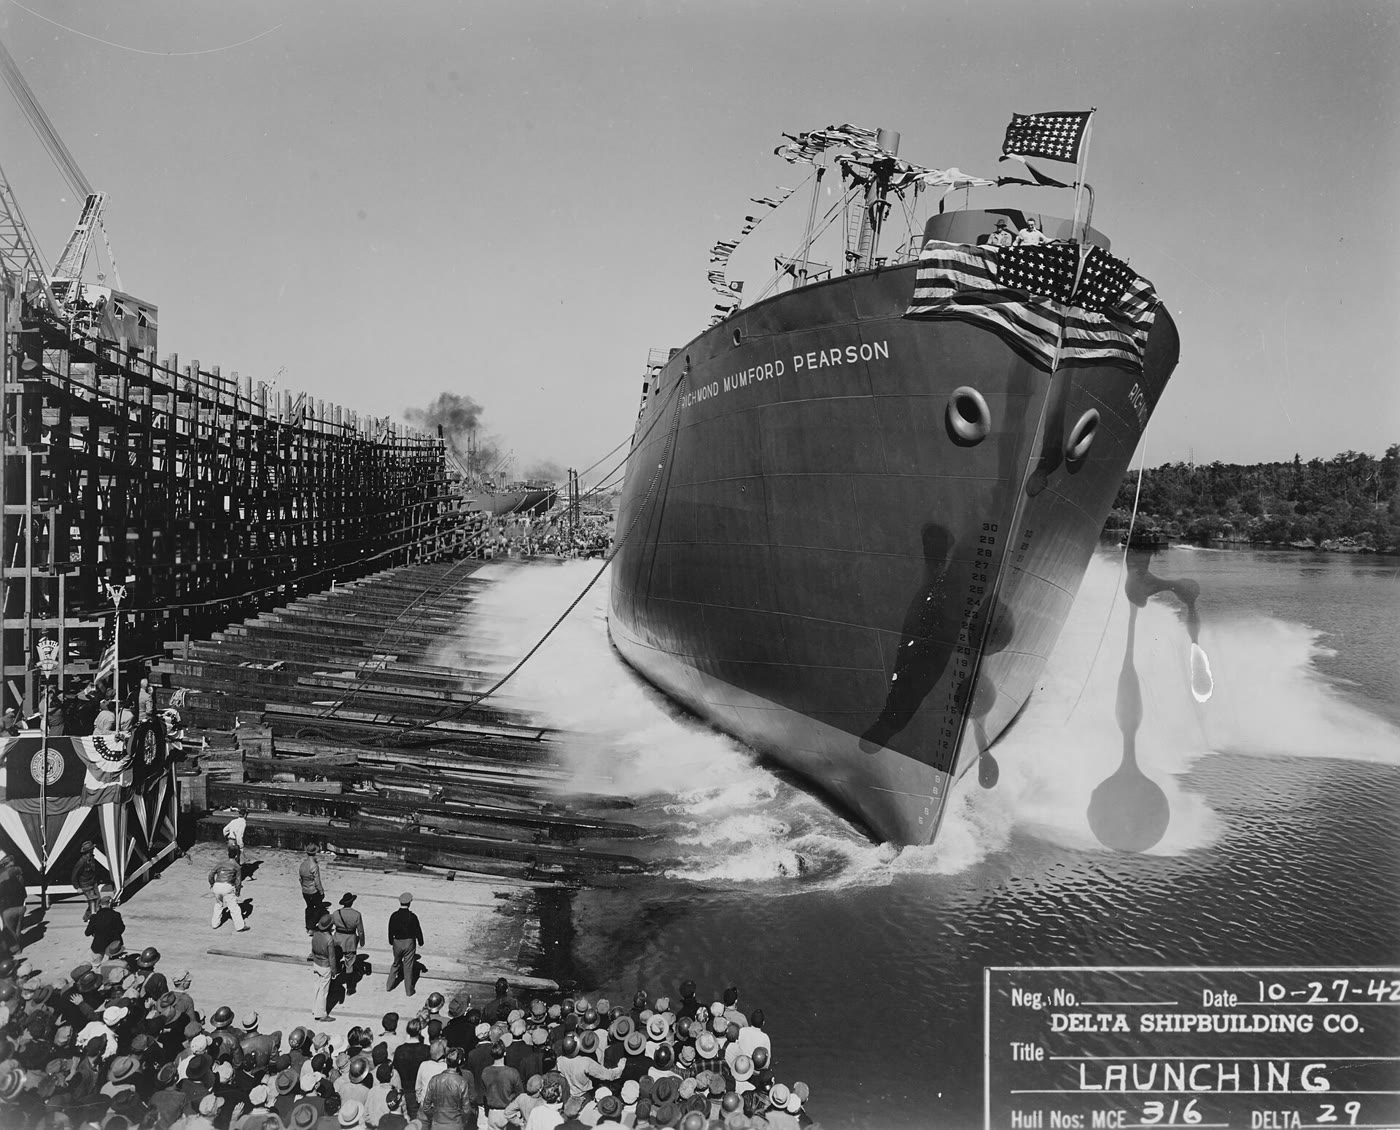
\includegraphics[width=0.58\linewidth]{images/book2/photos/g11-costs-liberty-ship-launch-1942.jpg}

{\small The launch of the Liberty ship \emph{Richmond Mumford Pearson} at a shipyard in New Orleans, 27 October 1942.}
\end{omfigure}

\section{Exercises}

\begin{exercise}[$\star$]\label{exo:g11:production-and-costs:1}
With 0 to 5 workers a workshop makes 0, 10, 25, 36, 44 and 48 tables a month. Compute the \omterm{def:g11:production-and-costs:marginal-product}{marginal product} of each worker. From which worker on is it diminishing?
\end{exercise}

\begin{exercise}[$\star$]\label{exo:g11:production-and-costs:2}
On a hectare of wheat, 0, 50, 100 and 150 kilograms of fertiliser give 2000, 2600, 3000 and 3200 kilograms of grain. Compute the \omterm{def:g11:production-and-costs:marginal-product}{marginal product} of fertiliser,
in kilograms of grain per kilogram of fertiliser, for each step.
\end{exercise}

\begin{exercise}[$\star$]\label{exo:g11:production-and-costs:3}
A firm's cost is $C(q) = 500 + 3q$. Compute the average fixed, average variable and \omterm{def:g11:production-and-costs:atc}{average total cost} at $q = 100$ and $q = 500$.
\end{exercise}

\begin{exercise}[$\star$]\label{exo:g11:production-and-costs:4}
A firm's total cost is 300, 400 and 600 dalens at 10, 20 and 30 units. Compute its \omterm{def:g11:production-and-costs:atc}{average total cost} at each, and the \omterm{def:g11:marginal-reasoning:marginal-benefit}{marginal cost} of each block of 10 units.
\end{exercise}

\begin{exercise}[$\star$]\label{exo:g11:production-and-costs:5}
Read the opening chart. About how much fertiliser per hectare and what yield do Kenya and the Netherlands show? Why can the chart not tell how much of Kenya's lower
yield is due to fertiliser?
\end{exercise}

\begin{exercise}[$\star\star$]\label{exo:g11:production-and-costs:6}
A firm's cost is $C(q) = 100 + 4q + q^2$. Write its \omterm{def:g11:marginal-reasoning:marginal-benefit}{marginal cost}, \omterm{def:g11:production-and-costs:atc}{average variable cost} and \omterm{def:g11:production-and-costs:atc}{average total cost}, and compute them at $q = 5$, $10$ and $20$.
\end{exercise}

\begin{exercise}[$\star\star$]\label{exo:g11:production-and-costs:7}
For the firm of \cref{exo:g11:production-and-costs:6}, find the output that makes \omterm{def:g11:production-and-costs:atc}{average total cost} lowest, using the derivative, and check that \omterm{def:g11:marginal-reasoning:marginal-benefit}{marginal cost}
equals \omterm{def:g11:production-and-costs:atc}{average total cost} there.
\end{exercise}

\begin{exercise}[$\star\star$]\label{exo:g11:production-and-costs:8}
The firm's fixed cost rises from 100 to 400. What happens to its \omterm{def:g11:marginal-reasoning:marginal-benefit}{marginal cost}, to its \omterm{def:g11:production-and-costs:atc}{average total cost}, and to the output that makes \omterm{def:g11:production-and-costs:atc}{average total cost} lowest?
\end{exercise}

\begin{exercise}[$\star\star$]\label{exo:g11:production-and-costs:9}
Read the fertiliser chart. Compute the rise in yield per quarter teaspoon for each of the three steps. Which dose earned the farmers the most, and why is it not the
dose that raised the yield most?
\end{exercise}

\begin{exercise}[$\star\star$]\label{exo:g11:production-and-costs:10}
The first unit of a new aircraft takes \num{100000} hours of labour, and production follows an 80\,\% \omterm{def:g11:production-and-costs:learning-curve}{learning curve}. How many hours do the 2nd, 4th, 8th and 64th units
take?
\end{exercise}

\begin{exercise}[$\star\star$]\label{exo:g11:production-and-costs:11}
At the yard of the record box, labour per ship fell from 1.73 million hours to about \num{406000}. By what percentage? With a \omterm{def:g11:production-and-costs:learning-curve}{learning curve} that cuts the hours by 20\,\%
per doubling, how many doublings of cumulative output would that take?
\end{exercise}

\begin{exercise}[$\star\star\star$]\label{exo:g11:production-and-costs:12}
What result of the Kenya trials would have contradicted \omterm{def:g11:production-and-costs:diminishing-mp}{diminishing marginal product}? Why does it matter that the doses were given at random to plots of the same
farms?
\end{exercise}

\begin{exercise}[$\star\star\star$]\label{exo:g11:production-and-costs:13}
Let $C(q) = F + aq + bq^2$ with $F$, $a$, $b > 0$. Show directly, by setting the derivative of $\mathit{ATC}$ to zero, that \omterm{def:g11:production-and-costs:atc}{average total cost} is lowest at $q^* = \sqrt{F/b}$,
that its lowest value is $a + 2\sqrt{Fb}$, and that \omterm{def:g11:marginal-reasoning:marginal-benefit}{marginal cost} equals it there.
\end{exercise}

\begin{exercise}[$\star\star\star$]\label{exo:g11:production-and-costs:14}
Three plant sizes have these \omterm{def:g11:production-and-costs:atc}{average total costs}, in kests a unit, at outputs of 10, 20, 30 and 40 units: small 12, 10, 14, 20; medium 16, 11, 9, 10; large 22, 15, 10,
8. Give the long-run average cost at each output and the plant used. Are there economies or \omterm{def:g11:production-and-costs:economies-of-scale}{diseconomies of scale} over this range? What can be said of the \omterm{def:g11:production-and-costs:mes}{minimum
efficient scale}?
\end{exercise}

\begin{exercise}[$\star\star\star$]\label{exo:g11:production-and-costs:15}
A firm's cost per unit has fallen over ten years while its output grew. Name two explanations that are not learning, and say what data would tell them apart.
\end{exercise}

\section{Problem: Kestria's Textile Mill}

\begin{problem}[{Weekend problem --- the cost family and the efficient scale of a mill}]
\label{pb:g11:production-and-costs:1}
A textile firm in Kestria can build a mill of three sizes. With output $q$ in thousands of metres of cloth a year, the yearly cost of each, in thousands of kests, is
\[
C_S(q) = 900 + 20q + 1.44q^2, \qquad C_M(q) = 3600 + 20q + 0.25q^2, \qquad C_L(q) = 8100 + 20q + 0.16q^2.
\]
So an average cost of $x$ (thousand kests per thousand metres) is $x$ kests a metre. The last figure of the chapter's long-run section shows the three average
cost curves.

\medskip
\noindent\textbf{Part I --- The cost family of the medium mill.}
\begin{enumerate}
\item Give the fixed cost and the variable cost of the medium mill at $q = 60$.
\item Compute its average fixed, average variable and \omterm{def:g11:production-and-costs:atc}{average total cost} at $q = 60$.
\item Write its \omterm{def:g11:marginal-reasoning:marginal-benefit}{marginal cost}, and compute it at $q = 60$.
\item At $q = 60$, is the \omterm{def:g11:production-and-costs:atc}{average total cost} rising or falling? Use \cref{prop:g11:marginal-reasoning:average}.
\item Where is the \omterm{def:g11:production-and-costs:atc}{average variable cost} lowest, and what is its value there?
\end{enumerate}

\medskip
\noindent\textbf{Part II --- The efficient output of the medium mill.}
\begin{enumerate}[resume]
\item Find, with the derivative, the output at which its \omterm{def:g11:production-and-costs:atc}{average total cost} is lowest.
\item Compute that lowest \omterm{def:g11:production-and-costs:atc}{average total cost}.
\item Check that \omterm{def:g11:marginal-reasoning:marginal-benefit}{marginal cost} equals it there.
\item Compute the \omterm{def:g11:production-and-costs:atc}{average total cost} at $q = 100$ and $q = 150$.
\item What is the lowest price at which the mill can cover all its costs?
\end{enumerate}

\medskip
\noindent\textbf{Part III --- Three plants.}
\begin{enumerate}[resume]
\item Find the output at which the small mill's \omterm{def:g11:production-and-costs:atc}{average total cost} is lowest, and its value there.
\item Same question for the large mill.
\item Which mill is cheapest per metre at $q = 40$? At $q = 200$?
\item Find the output at which the small and medium mills have the same \omterm{def:g11:production-and-costs:atc}{average total cost}.
\item Find the output at which the medium and large mills have the same \omterm{def:g11:production-and-costs:atc}{average total cost}.
\end{enumerate}

\medskip
\noindent\textbf{Part IV --- The long run.}
\begin{enumerate}[resume]
\item Describe the long-run average cost: which mill it follows on which range of output, and where it shows economies and \omterm{def:g11:production-and-costs:economies-of-scale}{diseconomies of scale}.
\item Give the \omterm{def:g11:production-and-costs:mes}{minimum efficient scale} and the lowest long-run average cost.
\item At a price of 80 kests a metre, buyers in Kestria want \num{600} thousand metres a year. How many mills of the efficient size could the market hold?
\item If buyers wanted only 100 thousand metres, which mill would be used, and at what average cost?
\item State the result of the problem: the \omterm{def:g11:production-and-costs:mes}{minimum efficient scale} and the minimum average cost.
\end{enumerate}
\end{problem}
